El t\'{e}rmino Aprendizaje Autom\'{a}tico se refiere a la detecci\'{o}n autom\'{a}tica de patrones significativos dentro de un conjunto de datos \cite{32}. En las \'{u}ltimas d\'{e}cadas se ha convertido en una herramienta com\'{u}n en casi cualquier tarea que requiera la extracci\'{o}n de informaci\'{o}n de gran cantidad de datos, por lo cual se ha convertido en una de las \'{a}reas de m\'{a}s r\'{a}pido crecimiento de la inform\'{a}tica.

\vspace{5mm} %5mm vertical space

Si bien el Aprendizaje Autom\'{a}tico puede resolver algunos problemas que son resueltos con algoritmos tradicionales, ha superado a \'{e}stos en problemas tales como el reconocimiento de im\'{a}genes, voz, lenguaje, escritura, juegos, rob\'{o}tica, an\'{a}lisis de datos, an\'{a}lisis de series de tiempo, etc. Desde esta perspectiva, se espera que mediante la aplicaci\'{o}n del Aprendizaje Autom\'{a}tico se pueda generar un modelo que se ajuste a un comportamiento normal esperado para un usuario.

\section{Aprendizaje Supervisado, Aprendizaje no Supervisado y Aprendizaje Semi-supervisado}

Existen diversas formas de clasificar los paradigmas de aprendizaje que existen, sin embargo en el presente trabajo s\'{o}lo se tratar\'{a}n el supervisado, el no supervisado y el semi-supervisado.

\vspace{5mm} %5mm vertical space

El \textbf{Aprendizaje Supervisado} es aquel que cuenta con variables de entrada (X) y una variable de salida (Y), este tipo de aprendizaje utiliza un algoritmo para aprender la funci\'{o}n de mapeo desde la entrada hasta la salida.

\begin{equation}
Y = f(X)
\end{equation}

El objetivo de este tipo de aprendizaje es aproximar la funci\'{o}n de mapeo de tal forma que cuando tenga datos de entrada nuevos (X) pueda predecir las variables de salida (Y) para esos datos. 

\vspace{5mm} %5mm vertical space

Este tipo de aprendizaje aborda dos tipos de problemas: clasificaci\'{o}n y regresi\'{o}n. Los problemas de \textbf{Clasificaci\'{o}n} son aquellos donde la variable de salida es una categor\'{i}a, como por ejemplo: ''Rojo'', ''Azul'', o ''Sano'', ''Enfermo'', por otra parte en los problemas de \textbf{Regresi\'{o}n} la variable de salida es un valor real, tal como: ''precio'' o ''altura''. Algunos de los tipos de problemas m\'{a}s comunes construidos sobre la clasificaci\'{o}n y la regresi\'{o}n incluyen la recomendaci\'{o}n y la predicci\'{o}n de series temporales.

\vspace{5mm} %5mm vertical space

Por otro lado el \textbf{Aprendizaje no Supervisado} es aquel donde s\'{o}lo se cuenta con datos de entrada (X) y no hay variables de salida correspondientes, su objetivo principal consiste en modelar la estructura o distribuci\'{o}n subyacente en los datos para aprender m\'{a}s acerca de los mismos.

\vspace{5mm} %5mm vertical space

En cuanto a los problemas del Aprendizaje sin supervisi\'{o}n, pueden ser agrupados en dos: agrupamiento y asociaci\'{o}n. El \textbf{Agrupamiento} es aquel donde se desea descubrir las agrupaciones inherentes en el conjunto de datos, como por ejemplo agrupar clientes por comportamiento de compra. Por otra parte la \textbf{Asociaci\'{o}n} es aquella que desea descubrir reglas que describen grandes porciones de sus datos, por ejemplo las personas que compran X tambi\'{e}n tienden a comprar Y. Algunos de los algoritmos de aprendizaje sin supervisi\'{o}n m\'{a}s populares son: K-means (para problemas de agrupamiento) y algoritmo Apriori (para problemas de aprendizaje de reglas de asociaci\'{o}n).

\vspace{5mm} %5mm vertical space

Por \'{u}ltimo se encuentra el \textbf{Aprendizaje Semi-supervisado}, el cual abarca aquellos problemas donde se tiene gran cantidad de datos de entrada (X) y s\'{o}lo algunos de los datos est\'{a}n etiquetados (Y). Este tipo de problemas se encuentran entre el aprendizaje supervisado y el no supervisado, adem\'{a}s es importante se\~{n}alar que muchos de los problemas de Aprendizaje Autom\'{a}tico en el mundo real se encuentran en esta \'{a}rea, esto debido a que resulta costoso o puede requerir mucho tiempo etiquetar el conjunto de datos, mientras que los datos no etiquetados son baratos, adem\'{a}s de ser f\'{a}ciles de recolectar y almacenar. Este tipo de problemas pueden usar una combinaci\'{o}n de t\'{e}cnicas supervisadas y no supervisadas para ser resueltos.

\vspace{5mm} %5mm vertical space

Dado que los m\'{e}todos de Aprendizaje Supervisado requieren una gran cantidad de datos de entrenamiento etiquetados, es importante aclarar que la recolecci\'{o}n de muestras negativas (conducci\'{o}n an\'{o}mala) es d\'{i}ficil y riesgosa para este estudio en particular; adem\'{a}s el enfoque supervisado presenta una limitaci\'{o}n potencial, la cual es: la detecci\'{o}n de nuevos patrones at\'{i}picos, esto debido a que el modelo resultante s\'{o}lo esta entrenado para reconocer un conjunto limitado de patrones an\'{o}malos, por lo cual al momento en que se presente un nuevo patr\'{o}n este modelo ser\'{a} incapaz de reconocerlo.

\vspace{5mm} %5mm vertical space

Por otra parte el enfoque sin supervisi\'{o}n tiene la ventaja de no requerir informaci\'{o}n etiquetada, sin embargo a menudo sufre altas tasas de falsas alarmas y bajas tasas de detecci\'{o}n \cite{33}. 

\vspace{5mm} %5mm vertical space

En muchas aplicaciones, incluyendo la del presente trabajo de grado, los ejemplos normales son f\'{a}ciles de conseguir, mientras que los an\'{o}malos son bastante dif\'{i}ciles de obtener, en consecuencia, para la realizaci\'{o}n de este estudio, se ha optado por la aplicaci\'{o}n del enfoque Semi-supervisado. De esta manera, como se mencion\'{o} en el Cap\'{i}tulo \ref{Capitulo 2}, el enfoque de \textbf{detecci\'{o}n de anomal\'{i}as Semi-supervisado} s\'{o}lo dispone de muestras normales en el conjunto de entrenamiento; es decir, no se puede obtener informaci\'{o}n sobre anomal\'{i}as, por lo tanto las muestras desconocidas se clasifican como valores at\'{i}picos, siempre y cuando su comportamiento sea muy diferente al de las muestras normales ya conocidas. Por lo tanto en este trabajo, se propone un m\'{e}todo de detecci\'{o}n de anomal\'{i}as de conducci\'{o}n semi-supervisado que consta de dos componentes: un modelo ajustado al comportamiento normal de manejo de un usuario y un m\'{e}todo de umbral para detecci\'{o}n de valores at\'{i}picos.

\vspace{5mm} %5mm vertical space

Para la generaci\'{o}n del modelo de detecci\'{o}n de anomal\'{i}as se opt\'{o} por algoritmos de aprendizaje autom\'{a}tico enfocados en series de tiempo, dado que los datos, de los sensores capturados por el dispositivo m\'{o}vil, dependen del tiempo en el que fueron capturados; por lo cual el primer paso a realizar es la generacion de peque\~{n}as fracciones de series temporales. En el Cuadro \ref{table:series-de-tiempo} se muestran los resultados de diferentes tama\~{n}os de series de tiempo.


\begin{landscape}
\pagestyle{empty}
\begin{table}[p!]

\centering
\begin{tabular}{|l|l|l|l|l|l|}
\hline
\multicolumn{1}{|c|}{\multirow{2}{*}{\textbf{\begin{tabular}[c]{@{}c@{}}Nro de \\ Componentes\end{tabular}}}} & \multicolumn{5}{c|}{\textbf{Tama\~{n}os de series de tiempo}}                                                                                                               \\ \cline{2-6} 
\multicolumn{1}{|c|}{}                                                                                        & \multicolumn{1}{c|}{\textbf{1}} & \multicolumn{1}{c|}{\textbf{2}} & \multicolumn{1}{c|}{\textbf{3}} & \multicolumn{1}{c|}{\textbf{4}} & \multicolumn{1}{c|}{\textbf{5}} \\ \hline
3                                                                              & \adj{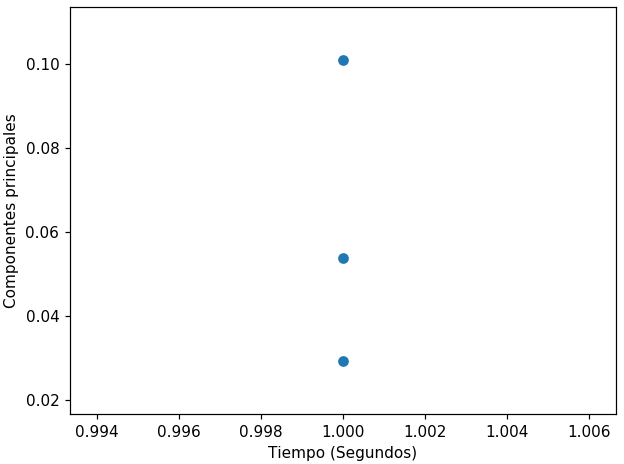
\includegraphics[width=1.5in]{imagenes/Cap4/pca3-1}} &\adj{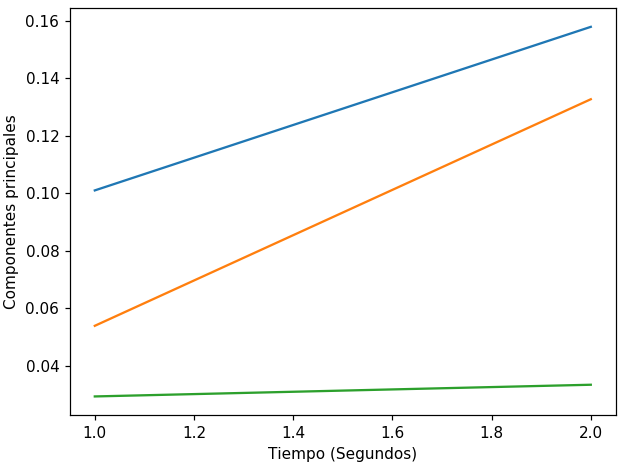
\includegraphics[width=1.5in]{imagenes/Cap4/pca3-2}}&\adj{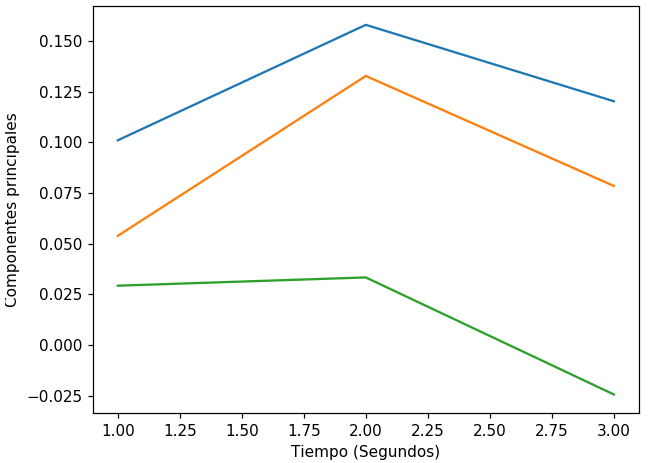
\includegraphics[width=1.5in]{imagenes/Cap4/pca3-3}}&\adj{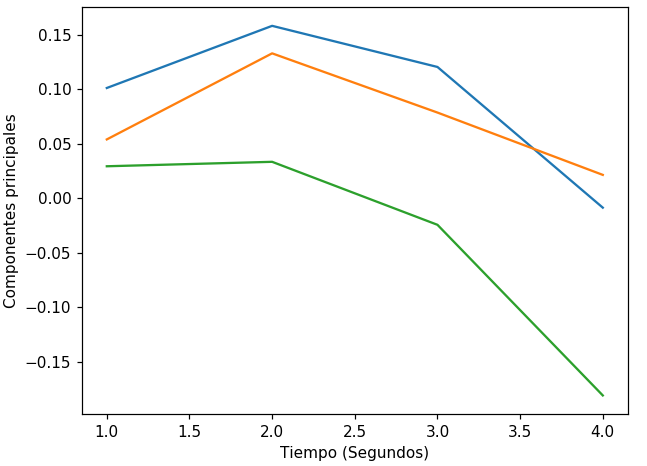
\includegraphics[width=1.5in]{imagenes/Cap4/pca3-4}}&\adj{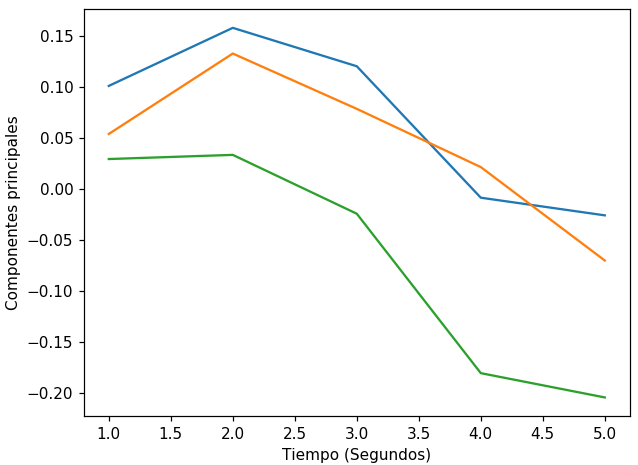
\includegraphics[width=1.5in]{imagenes/Cap4/pca3-5}} \\ \hline
4                                                                               & \adj{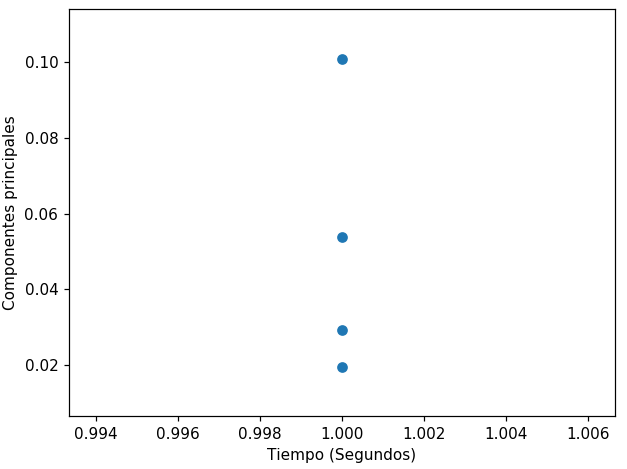
\includegraphics[width=1.5in]{imagenes/Cap4/pca4-1}} &\adj{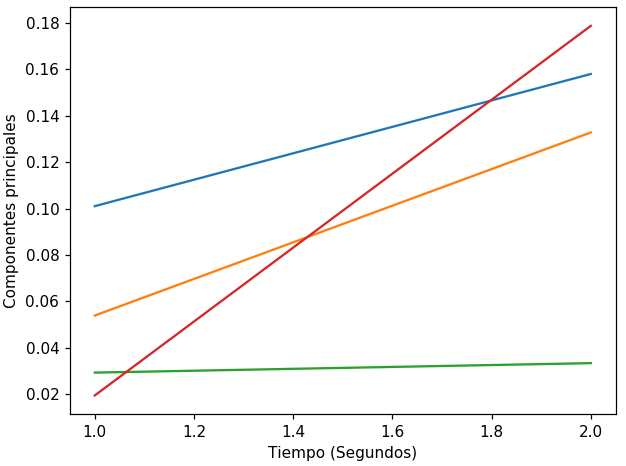
\includegraphics[width=1.5in]{imagenes/Cap4/pca4-2}}&\adj{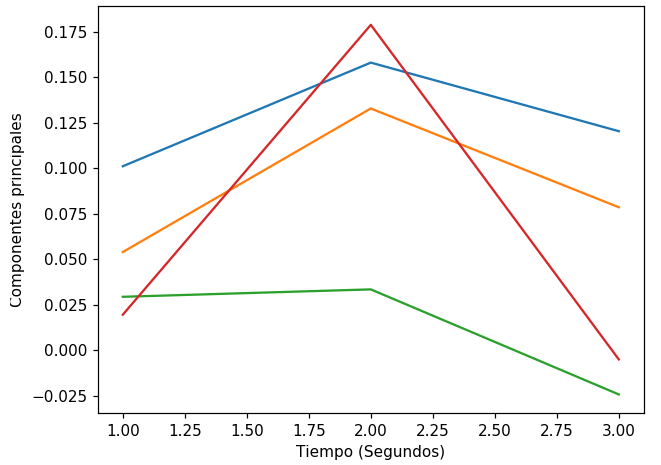
\includegraphics[width=1.5in]{imagenes/Cap4/pca4-3}}&\adj{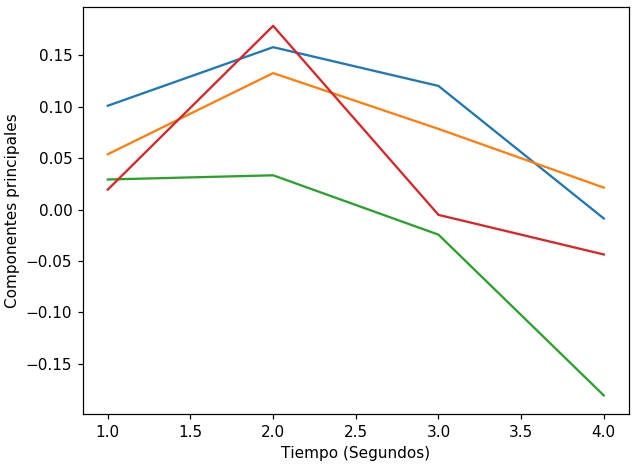
\includegraphics[width=1.5in]{imagenes/Cap4/pca4-4}}&\adj{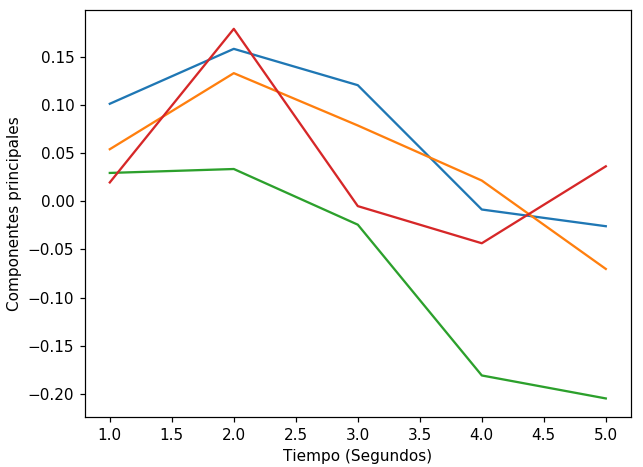
\includegraphics[width=1.5in]{imagenes/Cap4/pca4-5}} \\ \hline
\end{tabular}
\caption{Tabla con diferentes tama\~{n}os de series de tiempo para 3 y 4 componentes principales.}
  \label{table:series-de-tiempo}
\end{table}
\end{landscape}

\pagestyle{thesis}


 a continuaci\'{o}n se presenta algunos  algoritmos de aprendizaje autom\'{a}tico supervisado para series de tiempo.

\section{Aprendizaje autom\'{a}tico para an\'{a}lisis de series de tiempo}

Para entender la importancia de las series de tiempo se puede tomar la siguiente analog\'{i}a, los seres humanos no comienzan a pensar desde cero cada segundo, por lo que al leer un documento se comprende cada palabra bas\'{a}ndose en la comprensi\'{o}n de las palabras anteriores, es decir, no se elimina todo y se empieza a pensar de cero cada vez, dada \'{e}sta afirmaci\'{o}n se puede decir que los pensamientos de los seres humanos tienen persistencia.

\vspace{5mm} %5mm vertical space

Las redes neuronales tradicionales no tienen persistencia de los datos, lo que para algunos problemas en concreto, incluyendo el que se aborda en este trabajo, es una gran deficiencia. Con el fin de resolver este tipo de problemas aparecen las Redes Neuronales Recurrentes (RNN), las cuales son un tipo de red neuronal artificial propuesta en los a\~{n}os 80 (\cite{34}, \cite{35}, \cite{36}) dise\~{n}ada para reconocer patrones en secuencias de datos, como texto, genomas, escritura a mano, datos de series de tiempo num\'{e}ricos que emanan de sensores, entre otros.

\vspace{5mm} %5mm vertical space

La estructura de las RNN es similar a la de un perceptr\'{o}n multicapa \'{e}standar, con la diferencia de que permite conexiones entre unidades ocultas asociadas con un retardo de tiempo; a trav\'{e}s de estas conexiones, el modelo puede retener informaci\'{o}n sobre el pasado, lo que le permite descubrir correlaciones temporales entre eventos que est\'{a}n muy lejos unos de otros en los datos.

Las RNN tienen una cierta memoria de lo que sucedi\'{o} anteriormente en una secuencia de datos, esto ayuda al sistema a ganar contexto de los datos. Te\'{o}ricamente se dice que las RNN tiene memoria infinita, es decir, este tipo de redes tienen la capacidad de mirar hacia atras indefinidamente; sin embargo en la practica solo se puede mirar atras unos ultimos pasos.

LSTM esta dise\~{n}ado para obtener un flujo constante de errores en el tiempo y proteger este flujo de errores

